\chapter{线性方程组的直接解法}

求解线性代数方程组就相当于求解矩阵式$Ax=b$:
\begin{equation}
    \begin{bmatrix}
        a_{11}&\cdots&a_{1n}\\
        \vdots&\ddots&\vdots\\
        a_{n1}&\cdots&a_{nn}
    \end{bmatrix}\begin{bmatrix}
        x_1\\\vdots\\x_n
    \end{bmatrix}=\begin{bmatrix}
        b_1\\\vdots\\b_n
    \end{bmatrix}.
\end{equation}
因此有必要了解一些对矩阵的操作。

\section{矩阵操作}

\begin{definition}
    {稀疏矩阵}{sparse matrix}
    如果一个矩阵绝大多数元素是0,则称其是稀疏的(sparse)。
\end{definition}

\begin{definition}
    {秩一矩阵}{rank-1 matrix}
    若一个矩阵可以表示成$A=uv\dg$,则其秩为一。
\end{definition}

\begin{theorem}
    {奇异值分解}{singular value}
    根据奇异值分解,可以将矩阵表示成秩一矩阵的线性组合:
    \begin{equation}
        A=U\Sigma V\dg=\sum_i\sigma_iu_iv_i\dg,
    \end{equation}
    其中$U,V$为幺正矩阵。
\end{theorem}

\begin{theorem}
    {矩阵的Hierarchical表示}{Hierarchical matrix}
    考虑分块矩阵
    \[
        A=\begin{bmatrix}
            A_{11}&A_{12}\\
            A_{21}&A_{22}
        \end{bmatrix}
    \]
    $A$一般不是稀疏的,但非对角元$A_{12},A_{22}$是稀疏的,则$Ax$可以分块地写成:
    \[
        Ax=\begin{bmatrix}
            A_{11}&A_{12}\\
            A_{21}&A_{22}
        \end{bmatrix}\begin{bmatrix}
            x_1\\x_2
        \end{bmatrix}=\begin{bmatrix}
            A_{11}x_1+A_{12}x_2\\
            A_{21}x_1+A_{22}x_2
        \end{bmatrix},
    \]
    对$A_{11}x,A_{22}x_2$递归处理。
    \begin{center}
        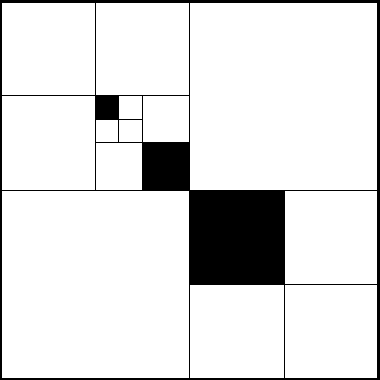
\includegraphics{figures/Hierarchical.pdf}
        \captionof{figure}{Hierarchical算法示意图,白块表示稀疏部分}
        \label{fig:Hierarchical}
    \end{center}
\end{theorem}

\begin{theorem}
    {矩阵乘法的Strassen算法}{}
    对矩阵乘法$C=AB$分块得:
    \[
        \begin{bmatrix}
            C_{11}&C_{12}\\
            C_{21}&C_{22}
        \end{bmatrix}=\begin{bmatrix}
            A_{11}&A_{12}\\
            A_{21}&A_{22}
        \end{bmatrix}\begin{bmatrix}
            B_{11}&B_{12}\\
            B_{21}&B_{22}
        \end{bmatrix},
    \]
    定义 
    \begin{subequations}
        \begin{align}
            M_1&=(A_{11}+A_{22})(B_{11}+B_{22}),\\
            M_2&=(A_{21}+A_{22})B_{11},\\
            M_3&=A_{11}(B_{12}-B_{22}),\\
            M_4&=A_{22}(B_{21}-B_{11}),\\
            M_5&=(A_{11}+A_{12})B_{22},\\
            M_6&=(A_{21}-A_{11})(B_{11}+B_{12}),\\
            M_7&=(A_{12}-A_{22})(B_{21}+B_{22}),
        \end{align}
    \end{subequations}
    则
    \begin{subequations}
        \begin{align}
            C_{11}&=M_1+M_4-M_5+M_7,\\
            C_{12}&=M_3+M_5,\\
            C_{21}&=M_2+M_4,\\
            C_{22}&=M_1-M_2+M_3+M_6.
        \end{align}
    \end{subequations}
    Strassen算法将分块矩阵的乘法从直接法的8次降低到了7次,由此分而治之,矩阵乘法的时间复杂度便从$\bigo(n^3)$降低到了$\bigo(n^{\log_27})=\bigo(n^{2.807})$。
\end{theorem}

\begin{definition}
    {离散Fourier变换}{discrete Fourier transform}
    式\eqref{eqn:Fourier betaj}中定义了一个线性变换,称为离散Fourier变换(discrete Fourier transform, DFT)
    \[
        X_n=\sum_{m=0}^{N-1}x_m\omega^{mn},
    \]
    其中$\omega:=\e{-\i2\pi/N}$是$N$次单位根,对应的变换矩阵为
    \begin{eqnarray}
        F=\begin{bmatrix}
            1&1&1&\cdots&1\\
            1&\omega&\omega^2&\cdots&\omega^{N-1}\\
            1&\omega^2&(\omega^2)^2&\cdots&(\omega^2)^{N-1}\\
            \vdots&\vdots&\vdots&\ddots&\vdots&\\
            1&\omega^{N-1}&(\omega^{N-1})^2&\cdots&(\omega^{N-1})^{N-1}
        \end{bmatrix}
    \end{eqnarray}
    事实上$F$上只有$n$个不同的元素。其逆变换为
    \begin{equation}
        F\iv=\frac1N\bar F.
    \end{equation}
\end{definition}

\begin{theorem}
    {Cooley-Tukey快速Fourier变换}{Cooley-Tukey fast Fourier transform}
    以基2 (radix-2)的情形为例,即$N=2^M$。
    将$X_n$的求和分成偶数项$E_n$和奇数项$O_n$
    \begin{align*}
        X_n&=\sum_{k=0}^{N/2-1}x_{2k}\omega^{2kn}+\sum_{k=0}^{N/2-1}x_{2k+1}\omega^{(2k+1)n}\\
        &=\sum_{k=0}^{N/2-1}x_{2k}\omega^{2kn}+\omega^n\sum_{k=0}^{N/2-1}x_{2k+1}\omega^{2kn}=:E_n+\omega^nO_n,
    \end{align*}
    由于$\omega^N=1$,注意到
    \begin{align*}
        X_{n+N/2}&=\sum_{k=0}^{N/2-1}x_{2k}\omega^{2k(n+N/2)}+\sum_{k=0}^{N/2-1}x_{2k+1}\omega^{(2k+1)(n+N/2)}\\
        &=\sum_{k=0}^{N/2-1}x_{2k}\omega^{2kn}-\omega^n\sum_{k=0}^{N/2-1}x_{2k+1}\omega^{2k}=E_n-\omega^nO_n,
    \end{align*}
    由此便将$N$个$X_n$求和($N^2$)转化成了$N/2$个$E_n,O_n$求和($N^2/2$)。
    采用分而治之的算法思想,可以将DFT的时间复杂度从矩阵向量乘法的$\bigo(N^2)$优化到$\bigo(N\log N)$,这称为快速Fourier变换(fast Fourier transform, FFT)。
    \begin{center}
        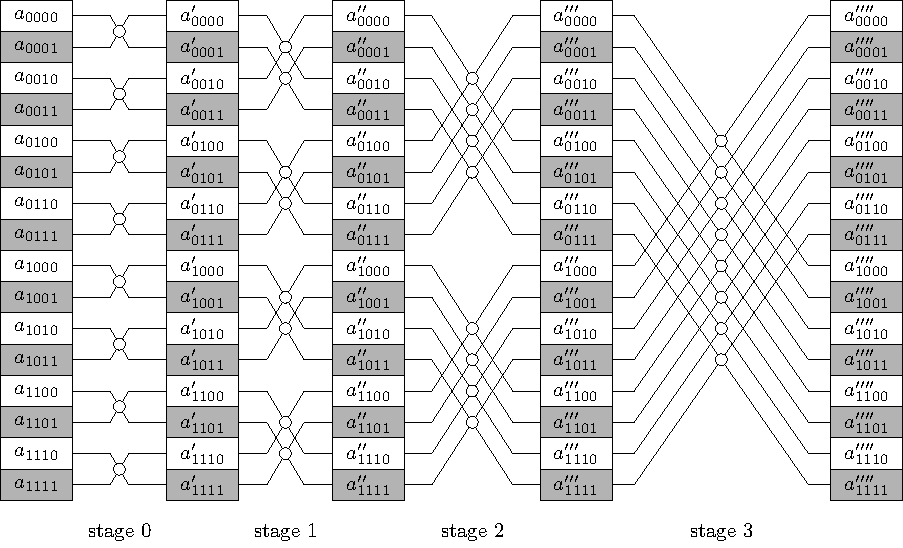
\includegraphics[width=0.8\linewidth]{figures/FFT.pdf}
        \captionof{figure}{FFT算法示意图($N=2^3=8$)}
        \label{fig:FFT}
    \end{center}
    \tcblower
    对于非基2的情形,$\omega^k$的周期不是基2的,做处理:
    \[
        X_n=\sum_{m=0}^{N-1}x_m\omega^{-mn}=\sum_{m=0}^Nx_m\omega^{[(m-n)^2-m^2-n^2]/2}.
    \]
    定义$\nu_k:=\omega^{k^2/2}$,记$Y_n:=\nu_nX_n,\;z_m:=\nu_m\iv x_m$,则有卷积形式:
    \[
        Y_n=\sum_{m=0}^{N-1}z_m\nu_{m-n}.
    \]
    可以用0将$z_m,\nu_m$延拓,使其周期是一个比$N$大的基2数$N'$。
    再在两端做DFT:
    \begin{align*}
        \sum_{n=0}^{N'-1}Y_n\omega_{N'}^{nk}&=\sum_{n=0}^{N'-1}\sum_{m=0}^{N'-1}z_m\nu_{m-n}\omega_{N'}^{nk}\\
        &=\sum_{m=0}^{N'-1}z_m\omega_{N'}^{mk}\sum_{n=0}^{N'-1}\nu_{m-n}\omega_{N'}^{(n-m)k}=\sum_{m=0}^{N'-1}z_m\omega_{N'}^{mk}\sum_{m=0}^{N'-1}\nu_m\omega_{N'}^{mk}
    \end{align*}
    因此通过对$z_m,\nu_m$做两次DFT、一次向量分量积、一次逆DFT便可得到$Y_n$。
\end{theorem}

\begin{theorem}
    {周期Toeplitz变换}{periodic Toeplitz transform}
    $n$阶矩阵$A$若满足$a_{ij}=c_{i-j}$且序列$c_k$周期为$n$,则$A$称为周期Toeplitz矩阵,且
    \begin{equation}
        A=F\iv\Lambda F,
    \end{equation}
    其中$\Lambda=\diag(\lambda_0,\ldots,\lambda_{n-1})$且
    \begin{equation}
        \lambda_i=\sum_{j=0}^{n-1}c_j\omega^{-ij}.
    \end{equation}
\end{theorem}

\begin{remark}
    $n$阶矩阵$A$若满足$a_{ij}=c_{i-j}$,则该矩阵可以扩展成$2n$阶的周期Toeplitz矩阵。
    \[
        \begin{bmatrix}
            A&*\\ *&*
        \end{bmatrix}
    \]
\end{remark}

\section{Gauss消元法}
\label{sec:Gauss elimination}

% \paragraph{基本思路}

% 将$Ax=b$的求解问题转化为一个与之等价的容易求解的问题$\tilde A\tilde x=\tilde b$。

\subsection{Gauss消元法}

如何求解$n$元线性方程组?
Cramer法则?时间复杂度$\bigo(n\cdot(n+1)!)$这是不可接受的。

\begin{theorem}
    {Gauss消元法}{Gauss elimination}
    线性方程组形如
    \begin{equation*}
        \lhkh{\begin{aligned}
            a_{11}^{(1)}x_1+a_{12}^{(1)}x_2+\cdots+a_{1n}^{(1)}x_n&=b_1^{(1)}\\
            a_{21}^{(1)}x_1+a_{22}^{(1)}x_2+\cdots+a_{2n}^{(1)}x_n&=b_2^{(1)}\\
            &\vdots\\
            a_{n1}^{(1)}x_1+a_{n2}^{(1)}x_2+\cdots+a_{nn}^{(1)}x_n&=b_n^{(1)}
        \end{aligned}}
    \end{equation*}
    如果$a_{11}^{(1)}\neq 0$,可将第一行的$-a_{i1}^{(1)}/a_{11}^{(1)}$倍加到第$i$行($i=2,3,\ldots,n$),得到一个等价方程组
    \begin{equation*}
        \lhkh{\begin{aligned}
            a_{11}^{(1)}x_1+a_{12}^{(1)}x_2+\cdots+a_{1n}^{(1)}x_n&=b_1^{(1)}\\
            a_{22}^{(2)}x_2+\cdots+a_{2n}^{(2)}x_n&=b_2^{(2)}\\
            &\vdots\\
            a_{n2}^{(2)}x_2+\cdots+a_{nn}^{(2)}x_n&=b_n^{(2)}
        \end{aligned}}
    \end{equation*}
    如果$a_{22}^{(2)}\neq 0$,便可以此类推……最终得到一个等价的上三角线性方程组:
    \begin{equation*}
        \lhkh{\begin{aligned}
            a_{11}^{(1)}x_1+a_{12}^{(1)}x_2+\cdots+a_{1n}^{(1)}x_n&=b_1^{(1)}\\
            a_{22}^{(2)}x_2+\cdots+a_{2n}^{(2)}x_n&=b_2^{(2)}\\
            &\vdots\\
            a_{nn}^{(n)}x_n&=b_n^{(n)}
        \end{aligned}}
    \end{equation*}
    便不难从下至上地解得:$x_n=b_n^{(n)}/a_{nn}^{(n)}$,
    \begin{equation}
        x_i=\division{\biggkh{b_{i}^{(i)}-\sum_{j=i+1}^na_{ij}^{(i)}x_j}}{a_{ii}^{(i)}},\quad i=n-1,\ldots,2,1.
    \end{equation}
    Gauss消元法的复杂度为$\bigo(n^3)$。
\end{theorem}

\begin{remark}
    从上面的算法过程中可见,
    一旦第$k$步$a_{kk}^{(k)}=0$,(顺序) Gauss消元法就不能继续进行下去。
    但是当第$k+1,\ldots,n$行中存在$a_{ik}^{k}\neq 0$,就可以交换$k,i$行,从而使算法继续。

    此外,即使$a_{kk}^{(k)}\neq 0$但$\abs{a_{kk}^{(k)}}\ll 1$,也会出现大数除小数导致精度下降的问题。
\end{remark}

\begin{theorem}
    {列主元方法}{pivoting technique}
    在第$k$步消去之前,找到绝对值最大的主元(pivot):
    \begin{equation}
        i_k=\mathop{\arg\max}\limits_{k\leq i\leq n}\abs{a_{ik}^{(k)}},
    \end{equation}
    然后交换第$k,i_k$行。
\end{theorem}

\subsection{LU分解}

下面我们从矩阵角度考察Gauss消元法。

\begin{definition}
    {初等矩阵}{elementary matrix}
    给定(实)向量$u,v$和标量$\sigma$,形如
    \begin{equation}
        E=I-\sigma uv\tp
    \end{equation}
    的称为(实)初等矩阵(elementary matrix)。
\end{definition}

\begin{corollary}
    初等矩阵的逆也是同类型的初等矩阵:
    \begin{equation}
        (I-\sigma uv\tp)\iv=I-\frac{\sigma}{\sigma v\tp u-1}uv\tp.
    \end{equation}
\end{corollary}

\begin{example}
    {}{}
    \begin{itemize}
        \item 初等排列矩阵:
        \[
            P_{ij}=I-(e_i-e_j)(e_i-e_j)\tp=I-e_{ii}-e_{jj}+e_{ij}+e_{ji}.
        \]
        左乘初等排列矩阵即互换第$i,j$行,右乘即互换第$i,j$列;
        \item 倍加矩阵:
        \[
            I+\alpha e_ie_j\tp=I+\alpha e_{ij},
        \]
        左乘即将第$i$行的$\alpha$倍加到第$j$行上。
    \end{itemize}
\end{example}

\begin{definition}
    {初等单位下三角矩阵}{elementary lower-triangle matrix}
    形如
    \begin{equation}
        L_i=I+\ell_ie_i\tp=\begin{bmatrix}
            1\\ &\ddots\\ &&1\\ &&\ell_{i+1,i}&1\\ &&\vdots&&\ddots\\ &&\ell_{ni}&&&1
        \end{bmatrix}
    \end{equation}
    称为第$i$列的初等单位下三角矩阵。其中向量$\ell_i$的前$i$个分量为0。
\end{definition}

\begin{corollary}
    初等单位下三角矩阵的逆也是初等单位下三角矩阵
    \begin{equation}
        (I+\ell_ie_i\tp)\iv=I-\ell_ie_i\tp.
    \end{equation}
\end{corollary}

\begin{corollary}
    对角元均为1的下三角矩阵称为单位下三角矩阵,可以写成
    \[
        L=L_1L_2\cdots L_{n-1}=\begin{bmatrix}
            1\\\ell_{21}&1\\ \vdots&\vdots&\ddots\\
            \ell_{n1}&\ell_{n2}&\cdots&1
        \end{bmatrix}.
    \]
\end{corollary}

\begin{theorem}
    {矩阵的LU分解}{LU decomposition exists}
    根据Gauss消元法的过程,记
    \[
        A^{(k)}:=\begin{bmatrix}
            a_{11}^{(1)}&\cdots&a_{1k}^{(1)}&\cdots&a_{1n}^{(1)}\\
            &\ddots&\vdots&\ddots&\vdots\\
            &&a_{kk}^{(k)}&\cdots&a_{kn}^{(k)}\\
            &&\vdots&\ddots&\vdots\\
            &&a_{nk}^{(k)}&\cdots&a_{nn}^{(k)}
        \end{bmatrix},\quad
        b^{(k)}:=\begin{bmatrix}
            b_1^{(1)}\\\vdots\\b_k^{(k)}\\\vdots\\b_n^{(k)}
        \end{bmatrix},\quad\ell_k:=-\frac1{a_{kk}^{(k)}}\begin{bmatrix}
            0\\\vdots\\0\\a_{k+1,k}^{(k)}\\\vdots\\a_{nk}^{(k)}
        \end{bmatrix}.
    \]
    相应的初等单位下三角矩阵为$L_k=I+\ell_ke_k\tp$。
    增广矩阵有递推关系:
    \begin{equation}
        [A^{(k+1)}\enspace b^{(k+1)}]=L_k[A^{(k)}\enspace b^{(k)}],
    \end{equation}
    即
    \[
        A^{(n)}=L_{n-1}\cdots L_1A^{(1)},\iff A^{(1)}=L_1\iv\cdots L_{n-1}\iv A^{(n)},
    \]
    则$L=L_1\iv\cdots L_{n-1}\iv$为单位下三角矩阵,$U=A^{(n)}$为上三角矩阵,这样就将$A^{(1)}$分解成了下上三角矩阵的乘积。    
\end{theorem}

\begin{remark}
    根据Gauss消元法的过程可见,LU分解的前提是$a_{11}^{(1)},\ldots,a_{nn}^{(n)}$均不为0。
\end{remark}

\begin{theorem}
    {三角分解定理}{LU decomposition}
    给定矩阵$A$,若其顺序主子式
    \begin{equation}
        \Delta_i:=\begin{vmatrix}
            a_{11}&\cdots&a_{1i}\\
            \vdots&\ddots&\vdots\\
            a_{i1}&\cdots&a_{ii}
        \end{vmatrix},\quad i=1,\ldots,n
    \end{equation}
    均不为0,则存在唯一的单位下三角矩阵$L$和上三角矩阵$U$使得$A=LU$。
\end{theorem}
\begin{proof}
    通过数学归纳法,可证明:$a_{11}^{(1)},\ldots,a_{ii}^{(i)}\neq 0\iff\Delta_1,\ldots,\Delta_i\neq 0$,此时
    \begin{equation}
        \Delta_i=a_{11}^{(1)}\cdots a_{ii}^{(i)},
    \end{equation}
    若存在$L_1,U_1$和$L_2,U_2$使得
    \[
        A=L_1U_1=L_2U_2,
    \]
    两边左乘$L_1\iv$,右乘$U_2\iv$得到:
    \[
        U_1U_2\iv=L_1\iv L_2,
    \]
    此式左边为上三角矩阵,右边为单位下三角矩阵,故只能是单位矩阵$I$,即$U_1=U_2,L_1=L_2$。
\end{proof}

\begin{example}
    {LU分解的例子}{}
    \[
        \begin{bmatrix}
            2&1&1&0\\4&3&3&1\\8&7&9&5\\6&7&9&8
        \end{bmatrix}=\begin{bmatrix}
            1\\2&1\\4&3&1\\3&4&1&1
        \end{bmatrix}\begin{bmatrix}
            2&1&1&0\\ &1&1&1\\ &&2&2\\ &&&2
        \end{bmatrix}.
    \]
\end{example}

\begin{remark}
    $L$有$n(n-1)/2$个变量,$U$有$n(n+1)/2$个变量,可以直接由$A$确定$L,U$。
\end{remark}

\begin{theorem}
    {直接LU分解法(Doolittle分解法)}{Doolittle decomposition}
    写成分块矩阵的形式:
    \[
        L^{(k)}=\begin{bmatrix}
            1\\\ell_{n-k+1}&L^{(k-1)}
        \end{bmatrix},\quad
        U^{(k)}=\begin{bmatrix}
            u_{u-k+1,u-k+1}&u_{u-k+1}\tp\\ &U^{(k-1)}
        \end{bmatrix},
    \]
    则
    \[
        A^{(k)}=L^{(k)}U^{(k)}=\begin{bmatrix}
            u_{u-k+1,u-k+1}&u_{u-k+1}\tp\\
            u_{u-k+1,u-k+1}\ell_{n-k+1}&A^{(k-1)}+\ell_{n-k+1}u_{u-k+1}\tp
        \end{bmatrix}.
    \]
    由此可确定$u,\ell$,同时$A^{(k)}$的阶数减1.
\end{theorem}
    
\begin{remark}
    三角分解\thmref{thm:LU decomposition} 给出了LU分解的条件。
    而对于一般的可逆矩阵,也可以通过换行实现LU分解。
\end{remark}

\begin{theorem}
    {一般三角分解定理}{LUP decomposition}
    若$A$可逆,则存在排列矩阵$P$、单位下三角矩阵$L$和上三角矩阵$U$使得
    \begin{equation}
        PA=LU.
    \end{equation}
\end{theorem}

\begin{proof}
    考虑列主元方法的Gauss消元法,第$k$步交换$k,i_k$行,则
    \[
        A^{(k+1)}=L_kI_{ki_k}A^{(k)},
    \]
    即
    \[
        A^{(n)}=L_{n-1}I_{n-1,i_{n-1}}\cdots L_1I_{1i_1}A^{(1)},
        \iff
        A^{(1)}=I_{1i_1}L_1\iv\cdots I_{n-1,i_{n-1}}L_{n-1}\iv A^{(n)},
    \]
    定义
    \[
        P_k=I_{n-1,i_{n-1}}\cdots I_{ki_k},
    \]
    则$P_k\tp P_{k+1}=I_{ki_k}$,进而
    \[
        P_1A^{(1)}=P_2L_1\iv P_2\tp P_3L_2\iv\cdots P_{n-1}L_{n-1}\iv A^{(n)},
    \]
    易得$P_{k+1}e_k=e_k$,故
    \[
        L_k':=P_{k+1}L_k\iv P_{k+1}\tp=P_{k+1}(I-\ell_ke_k\tp)P_{k+1}\tp=I-P_{k+1}\ell_ke_k\tp,
    \]
    仍然是第$k$列的初等单位上三角矩阵,
    令$P=P_1,\;L=L_1'\cdots L_{n-2}'L_{n-1},\;U=A^{(n)}$即得。
\end{proof}

\subsection{Cholesky分解}

下面再看对称矩阵的三角分解。

\begin{theorem}
    {Cholesky分解}{Cholesky decomposition}
    若$A$实对称正定,则存在唯一的对角元素为正的下三角矩阵$L$使得
    \begin{equation}
        A=LL\tp.
    \end{equation}
\end{theorem}

\begin{proof}
    采用加边Cholesky分解法:写成分块矩阵的形式
    \[
        L_i=\begin{bmatrix}
            L_{i-1}\\\ell_{i-1}\tp&\ell_{ii}
        \end{bmatrix},\quad A_i=\begin{bmatrix}
            A_{i-1}&a_{i-1}\\ a_{i-1}\tp&a_{ii}
        \end{bmatrix}
    \]
    满足$A_i=L_iL_i\tp$,
    可得 
    \begin{subequations}
        \begin{align}
            \ell_{i-1}&=L_{i-1}\iv a_{i-1},\\
            \ell_{ii}&=\sqrt{a_{ii}-\ell_{i-1}\tp\ell_{i-1}}.
        \end{align}
    \end{subequations}
    从$\ell_{11}=\sqrt{a_{11}}$出发便可迭代得到整个$L$。
\end{proof}

\begin{remark}
    这种算法特别适合稀疏矩阵。
\end{remark}

\subsection{Thomas方法}

考虑线性方程组
\[
    \begin{cases}
        b_1x_1+c_1x_2=d_1,\\
        a_ix_{i-1}+b_ix_i+c_ix_{i+1}=d_i,&i=2,\ldots,n-1\\
        a_nx_{n-1}+b_nx_n=d_n
    \end{cases}
\]
系数矩阵为三对角矩阵:
\[
    \begin{bmatrix}
        b_1&c_1\\a_2&b_2&\ddots\\ &\ddots&\ddots&c_{n-1}\\ &&a_n&b_b
    \end{bmatrix}.
\]
\begin{theorem}
    {Thomas方法}{Thomas technique}
    容易验证有如下三角分解形式:
    \[
        A=LU=\begin{bmatrix}
            1\\\ell_2&1\\&\ddots&\ddots\\ &&\ell_n&1
        \end{bmatrix}\begin{bmatrix}
            u_1&c_1\\ &u_2&\ddots\\ &&\ddots&c_{n-1}\\ &&&u_n
        \end{bmatrix},
    \]
    可直接乘开得到$u_1=b_1$
    \begin{equation}
        \ell_i=\frac{a_i}{u_{i-1}},\quad u_i=b_i-\ell_ic_{i-1}.
    \end{equation}
\end{theorem}


\section{稳定性分析}
\label{sec:stability analysis}

在用直接法求解$Ax=b$的过程中,由于舍入误差的存在,必然会导致结果产生误差。因而有必要对可能产生的误差作一估计。
% 通常我们假设在数值处理的过程中计算都是精确的.
\begin{example}
    {数据的微小变化导致解的巨大变化}{}
    方程组
    \[
        \begin{bmatrix}
            10&7&8&7\\
            7&5&6&5\\
            8&6&10&9\\
            7&5&9&10
        \end{bmatrix}\begin{bmatrix}
            x_1\\x_2\\x_3\\x_4
        \end{bmatrix}=\begin{bmatrix}
            32\\23\\33\\31
        \end{bmatrix}\implies\begin{bmatrix}
            x_1\\x_2\\x_3\\x_4
        \end{bmatrix}=\begin{bmatrix}
            1\\1\\1\\1
        \end{bmatrix}.
    \]
    对向量$b$数据做微小的修改
    \[
        \begin{bmatrix}
            10&7&8&7\\
            7&5&6&5\\
            8&6&10&9\\
            7&5&9&10
        \end{bmatrix}\begin{bmatrix}
            x_1'\\x_2'\\x_3'\\x_4'
        \end{bmatrix}=\begin{bmatrix}
            32.1\\22.9\\33.1\\30.9
        \end{bmatrix}\implies\begin{bmatrix}
            x_1'\\x_2'\\x_3'\\x_4'
        \end{bmatrix}=\begin{bmatrix}
            9.2\\-12.6\\4.5\\-1.1
        \end{bmatrix}.
    \]
    对系数矩阵$A$数据做微小的修改
    \[
        \begin{bmatrix}
            10&7&8.1&7.2\\
            7.08&5.04&6&5\\
            8&5.98&9.89&9\\
            6.99&4.99&9&9.98
        \end{bmatrix}\begin{bmatrix}
            x_1''\\x_2''\\x_3''\\x_4''
        \end{bmatrix}=\begin{bmatrix}
            32\\23\\33\\31
        \end{bmatrix}\implies\begin{bmatrix}
            x_1''\\x_2''\\x_3''\\x_4''
        \end{bmatrix}=\begin{bmatrix}
            -81\\137\\-34\\22
        \end{bmatrix}.
    \]
    可见数据的微小变化会导致解的巨大变化,这是因为系数矩阵的条件数$\cond(A)=32825/11$很大。
\end{example}

\begin{definition}
    {条件数}{condition number}
    给定诱导的矩阵范数$\norm\cdot$,可逆矩阵$A$的条件数(condition number)为
    \begin{equation}
        \cond(A)\equiv\norm A\nnorm{A\iv}.
    \end{equation}
\end{definition}

\begin{corollary}
    条件数的性质:
    \begin{itemize}
        \item $\cond(A)\geq 1$;
        \item $\cond(A\iv)=\cond(A)$;
        \item $\cond(cA)=\cond(A)$;
        \item 若$U$为正交矩阵,则$\cond_2(U)=1$,且
        \begin{equation}
            \cond_2(A)=\cond_2(AU)=\cond_2(UA);
        \end{equation}
        \item 若$\lambda_1,\lambda_n$是$A$模最大与最小的特征值,则
        \begin{equation}
            \cond(A)\geq\frac{\abs{\lambda_1}}{\abs{\lambda_n}},
        \end{equation}
        若$A$对称,则$\cond_2(A)=\abs{\lambda_1}/\abs{\lambda_n}$;
        \item 由范数的等价性,可知条件数的等价性:
        \begin{subequations}
            \begin{alignat}{4}
                \frac1n&\cond_2&(A)&\leq\cond_1&(A)&\leq n\cond_2&(A),\\
                \frac1n&\cond_\infty&(A)&\leq\cond_2&(A)&\leq n\cond_\infty&(A),\\
                \frac1{n^2}&\cond_1&(A)&\leq\cond_\infty&(A)&\leq n^2\cond_1&(A).
            \end{alignat}
        \end{subequations}
    \end{itemize}
\end{corollary}

\begin{theorem}
    {解的扰动定理}{}
    给定可逆矩阵$A$和微小扰动$\D A$,满足
    \[
        \frac{\norm{\D A}}{\norm A}<\frac1{\cond(A)},
    \]
    则$(A+\D A)$也可逆,考察线性方程组$Ax=b$及其扰动方程组
    \[
        (A+\D A)(x+\D x)=b+\D b,
    \]
    则有
    \begin{equation}
        \frac{\norm{\D x}}{\norm x}\leq\frac{\cond(A)}{1-\norm{A\iv}\norm{\D A}}\biggkh{\frac{\norm{\D A}}{\norm A}+\frac{\norm{\D b}}{\norm b}}.
    \end{equation}
\end{theorem}

\begin{proof}
    由扰动定理\thmref{thm:perturbation theorem II} 知$(A+\D A)$可逆且
    \begin{equation}
        \norm{(A+\D A)\iv}\leq\frac{\norm{A\iv}}{1-\norm{A\iv}\norm{\D A}}.
    \end{equation}
    由
    \begin{align*}
        \D x&=(A+\D A)\iv(b+\D b)-x\\
        &=(A+\D A)\iv(b+\D b-(A+\D A)x)\\
        &=(A+\D A)\iv(\D b-\D Ax),
    \end{align*}
    两边取范数
    \begin{align*}
        \norm{\D x}&\leq\norm{(A+\D A)\iv}(\norm{\D b}+\norm{\D A}\norm x)\\
        &\leq\frac{\norm{A\iv}}{1-\norm{A\iv}\norm{\D A}}\biggkh{\frac{\norm{\D A}}{\norm A}\norm A\norm x+\frac{\norm{\D b}}{\norm b}\norm A\norm x}.
        \qedhere
    \end{align*}
\end{proof}

\begin{remark}
    因此条件数可以看成扰动方程组相对误差的放大倍数。
\end{remark}

\begin{theorem}
    {矩阵相对奇异性的度量}{relative singularity}
    若$A$可逆,定义所有使得$(A+\D A)$不可逆的$\D A$构成集合$S$,则 
    \begin{equation}
        \min_{\D A\in S}\frac{\norm{\D A}_2}{\norm A_2}=\frac1{\cond_2(A)},
    \end{equation}
\end{theorem}

\begin{proof}
    当$\nnorm{A\iv}\norm{\D A}<1$时,$(A+\D A)$可逆,故
    \[
        \min_{\D A\in S}\norm{\D A}_2\geq\frac1{\norm{A\iv}_2}.
    \]
    由$\norm\cdot_2$的定义,$\exists x$且$\norm x_2=1$使得$\norm{A\iv x}_2=\norm{A\iv}_2$,令$y=A\iv x/\nnorm{A\iv}_2$,并取
    \[
        \D A=-\frac{xy\tp}{\norm{A\iv}_2},
    \]
    则$\norm y_2=1$且
    \[
        (A+\D A)y=\frac{x}{\norm{A\iv}_2}-\frac{xy\tp y}{\norm{A\iv}_2}=0,
    \]
    故$(A+\D A)$不可逆,又
    \[
        \norm{\D A}_2=\max_{\norm z_2=1}\norm{\D Az}_2=\frac{\norm x_2}{\norm{A\iv}_2}\max_{\norm z_2=1}\abs{y\tp z}=\frac1{\norm{A\iv}_2}.
        \qedhere
    \]
\end{proof}

\begin{remark}
    因此可逆矩阵到最接近的奇异矩阵的相对距离在2 - 范数意义下就是2 - 条件数的倒数。当条件数很大时,矩阵与奇异矩阵的相对距离很小,称为病态(ill conditioned)。
\end{remark}

\begin{theorem}
    {近似解的相对误差}{}
    若$x,x'$分别是方程组$Ax=b$的精确解和近似解,$x'$的剩余$r=b-Ax'$,则
    \begin{equation}
        \frac1{\cond(A)}\frac{\norm r}{\norm b}\leq\frac{\norm{x'-x}}{\norm x}\leq\cond(A)\frac{\norm r}{\norm b}.
    \end{equation}
\end{theorem}

\begin{proof}
    由$A(x'-x)=-r$和$\norm A\norm x\geq\norm b$可得
    \[
        \norm r\leq\norm A\norm{x'-x}=\frac{\cond(A)}{\norm{A\iv}}\norm{x'-x},
    \]
    两边除$\norm b$,由$x=A\iv b$可得 
    \[
        \frac{\norm r}{\norm b}\leq\cond(A)\frac{\norm{x'-x}}{\norm{A\iv}\norm b}\leq\cond(A)\frac{\norm{x'-x}}{\norm x};
    \]
    另一方面,由$x'-x=-A\iv r$可得
    \[
        \norm{x'-x}=\norm{A\iv r}\leq\norm{A\iv}\norm r=\cond(A)\frac{\norm r}{\norm A}.
    \]
    两边同除$\norm x$,由$Ax=b$可得 
    \[
        \frac{\norm{x'-x}}{\norm x}\leq\cond(A)\frac{\norm r}{\norm A\norm x}\leq\cond(A)\frac{\norm r}{\norm b}.
    \]
    综上,两边不等式均得证。
\end{proof}

\begin{remark}
    这说明当方程组病态时,即使剩余$\norm r$比较小,解的相对误差仍可能很大。
\end{remark}

\begin{example}
    {Hilbert矩阵}{Hilbert matrix}
    Hilbert矩阵
    \begin{equation*}
        H_n:=\begin{bmatrix}
            1&1/2&\cdots&1/(n+1)\\
            1/2&1/3&\cdots&1/(n+2)\\
            \vdots&\vdots&\ddots&\vdots\\
            1/(n+1)&1/(n+2)&\cdots&1/(2n+1)
        \end{bmatrix}
    \end{equation*}
    的条件数增长很快:
    \[
        \cond_2(H_n)=\bigo\biggkh{\frac{(1+\sqrt2)^{4n}}{\sqrt n}}.
    \]
\end{example}

\begin{theorem}
    {条件数与数值精度}{}
    用直接法解方程组$Ax=b$,$A,b$的元素有效位数为$s$而$\cond(A)$的数量级为$t$,则求得$x$分量有效位数约为$s-t$。
\end{theorem}

\paragraph{病态方程组的解法}

除采用更高精度的运算外,另一个更有效的方法是对原方程进行预处理:
\[
    Ax=b,\iff PAQ(Q\iv x)=Pb,
\]
从而降低系数矩阵的条件数:$\cond(PAQ)\ll\cond(A)$。一般$P,Q$可选择为三角矩阵或对角矩阵。

\begin{example}
    {预处理例子}{}
    方程组
    \[
        \begin{bmatrix}
            10&10^5\\1&1
        \end{bmatrix}\begin{bmatrix}
            x_1\\x_2
        \end{bmatrix}=\begin{bmatrix}
            10^5\\2
        \end{bmatrix}\implies\begin{bmatrix}
            x_1\\x_2
        \end{bmatrix}=\frac1{9999}\begin{bmatrix}
            10000\\9998
        \end{bmatrix}.
    \]
    系数矩阵的条件数$\cond_2(A)=100010$很大,左乘$D=\diag(10^{-5},1)$平衡:
    \[
        \begin{bmatrix}
            10^{-4}&1\\1&1
        \end{bmatrix}\begin{bmatrix}
            x_1\\x_2
        \end{bmatrix}=\begin{bmatrix}
            1\\2
        \end{bmatrix},
    \]
    系数矩阵的条件数$\cond_2(DA)=940/359$得到了有效降低。
\end{example}
